\documentclass[tikz,border=8pt]{standalone}
\usepackage{amsmath}
\usepackage{amssymb}
\usetikzlibrary{arrows.meta}
\usetikzlibrary{calc}
\usetikzlibrary{decorations.pathreplacing}
\usetikzlibrary{decorations.pathmorphing}
\usetikzlibrary{patterns}
\usetikzlibrary{shapes.geometric}
\usetikzlibrary{positioning}
\usetikzlibrary{shadings}

\begin{document}
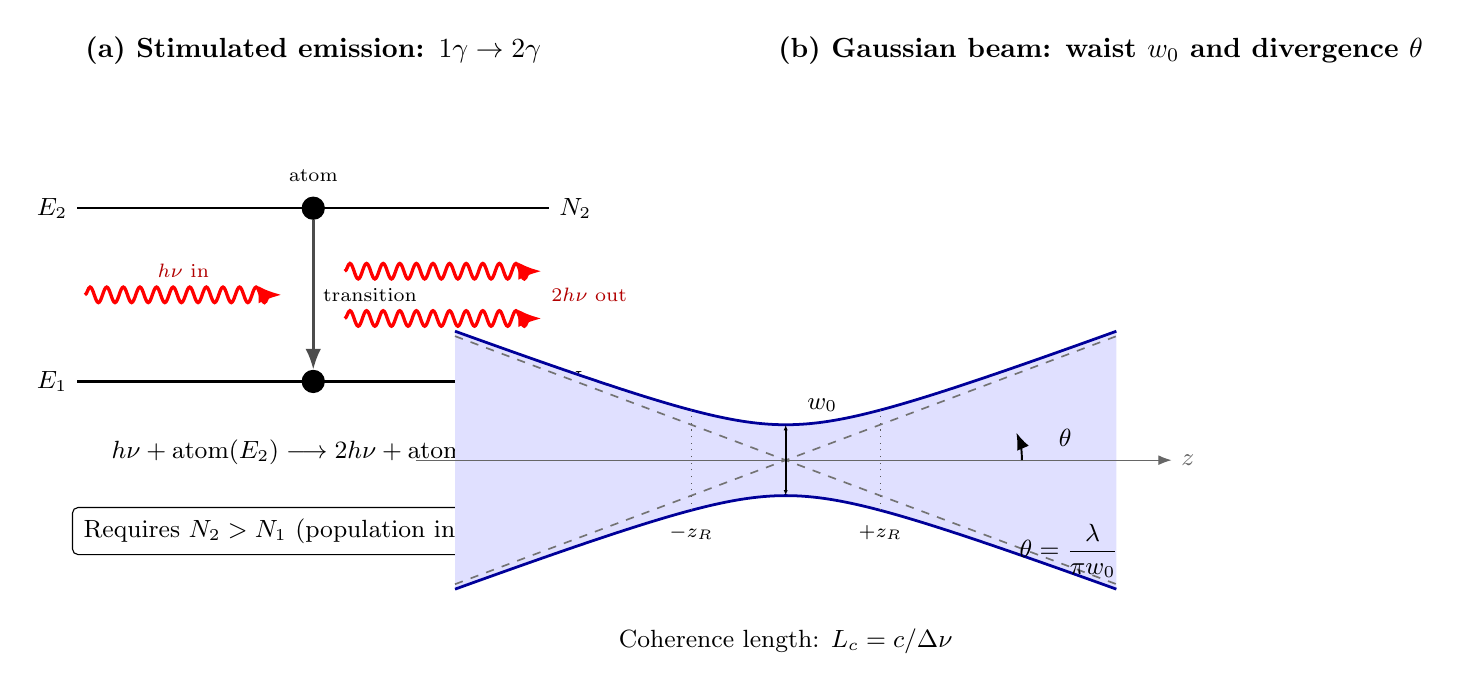
\begin{tikzpicture}[>=Latex]

% ============================================================
% Panel (a): Stimulated emission, level diagram, one-to-two
% ============================================================
\begin{scope}[shift={(0,0)}]

  % Panel title
  \node[font=\bfseries] at (3.5,5.2) {(a) Stimulated emission: $1\gamma \to 2\gamma$};

  % Energy levels
  \draw[line width=0.8pt] (0.5,1.0) -- (6.5,1.0);     % E1 (ground)
  \draw[line width=0.8pt] (0.5,3.2) -- (6.5,3.2);     % E2 (excited)

  % Level labels
  \node[left, font=\small] at (0.5,1.0) {$E_1$};
  \node[left, font=\small] at (0.5,3.2) {$E_2$};

  % Population labels
  \node[right, font=\small] at (6.5,1.0) {$N_1$};
  \node[right, font=\small] at (6.5,3.2) {$N_2$};

  % Atom on E2 (before): filled circle
  \filldraw[black] (3.5,3.2) circle (4.0pt);
  \node[above=2pt, font=\scriptsize] at (3.5,3.35) {atom};

  % Incoming photon (red wave, left -> atom)
  \draw[red, line width=1.2pt, decorate, decoration={snake, amplitude=2.8pt, segment length=6pt, post length=4pt}, ->]
        (0.6,2.1) -- (3.1,2.1);
  \node[above, font=\scriptsize, red!70!black] at (1.85,2.2) {$h\nu$ in};

  % Transition arrow from E2 to E1
  \draw[->, line width=1.0pt, black!70] (3.5,3.05) -- (3.5,1.15);
  \node[right, font=\scriptsize] at (3.5,2.1) {transition};

  % Atom on E1 (after)
  \filldraw[black] (3.5,1.0) circle (4.0pt);

  % Two outgoing cloned photons (red waves, same phase, same direction)
  \draw[red, line width=1.2pt, decorate, decoration={snake, amplitude=2.8pt, segment length=6pt, post length=4pt}, ->]
        (3.9,2.4) -- (6.4,2.4);
  \draw[red, line width=1.2pt, decorate, decoration={snake, amplitude=2.8pt, segment length=6pt, post length=4pt}, ->]
        (3.9,1.8) -- (6.4,1.8);
  \node[right, font=\scriptsize, red!70!black] at (6.4,2.1) {$2h\nu$ out};

  % Process formula (below)
  \node[font=\small] at (3.5,0.1) {$h\nu + \mathrm{atom}(E_2) \longrightarrow 2h\nu + \mathrm{atom}(E_1)$};

  % Inversion condition (boxed)
  \node[draw, rounded corners=2pt, font=\small, inner sep=4pt] at (3.5,-0.9) {Requires $N_2 > N_1$ (population inversion)};

\end{scope}

% ============================================================
% Panel (b): Gaussian beam waist and far-field divergence
% ============================================================
\begin{scope}[shift={(9.5,0)}]

  % Panel title
  \node[font=\bfseries] at (4.0,5.2) {(b) Gaussian beam: waist $w_0$ and divergence $\theta$};

  % Parameters for the hyperbolic envelope w(z) = w0 * sqrt(1+(z/zR)^2)
  % Use w0 = 0.45, zR = 1.2, x in [-4.2, 4.2]
  % Far-field asymptote slope = w0/zR = 0.375

  % Shaded interior (light blue) bounded by +w(z) and -w(z)
  \fill[blue!12, domain=-4.2:4.2, samples=121, variable=\x]
        plot ({\x}, {0.45*sqrt(1+(\x/1.2)^2)})
        -- plot[domain=4.2:-4.2] ({\x}, {-0.45*sqrt(1+(\x/1.2)^2)})
        -- cycle;

  % Upper envelope (hyperbola) - dark blue
  \draw[blue!60!black, line width=1.0pt, domain=-4.2:4.2, samples=121, variable=\x]
        plot ({\x}, {0.45*sqrt(1+(\x/1.2)^2)});

  % Lower envelope (hyperbola) - dark blue
  \draw[blue!60!black, line width=1.0pt, domain=-4.2:4.2, samples=121, variable=\x]
        plot ({\x}, {-0.45*sqrt(1+(\x/1.2)^2)});

  % Horizontal axis (propagation axis z)
  \draw[->, thin, black!60] (-4.7,0) -- (4.9,0) node[right, font=\small] {$z$};

  % Far-field asymptotes (dashed)
  \draw[dashed, black!55, line width=0.6pt] (-4.2,-1.575) -- (4.2,1.575);
  \draw[dashed, black!55, line width=0.6pt] (-4.2,1.575)  -- (4.2,-1.575);

  % Waist marker at z=0
  \draw[{Latex[length=2pt]}-{Latex[length=2pt]}, line width=0.7pt] (0,-0.45) -- (0,0.45);
  \node[right, font=\small] at (0.15,0.7) {$w_0$};

  % Rayleigh length markers at z = +/- zR = +/- 1.2
  \draw[dotted, black!65] (1.2,-0.636) -- (1.2,0.636);
  \draw[dotted, black!65] (-1.2,-0.636) -- (-1.2,0.636);
  \node[font=\scriptsize, below] at (1.2,-0.7) {$+z_R$};
  \node[font=\scriptsize, below] at (-1.2,-0.7) {$-z_R$};

  % Divergence angle theta at far field
  \draw[->, line width=0.7pt] (3.0,0) arc (0:23:0.9);
  \node[font=\small] at (3.55,0.28) {$\theta$};

  % Theta formula
  \node[font=\small] at (3.6,-1.15) {$\theta = \dfrac{\lambda}{\pi w_0}$};

  % Coherence-length note
  \node[font=\small] at (0,-2.3) {Coherence length: $L_c = c/\Delta\nu$};

\end{scope}

\end{tikzpicture}
\end{document}
